\documentclass[12pt]{article}
\usepackage[T1]{fontenc}
\usepackage[T1]{polski}
\usepackage[utf8]{inputenc}
\newcommand{\BibTeX}{{\sc Bib}\TeX} 
\usepackage{graphicx}
\usepackage{amsfonts}
\usepackage{listings}
\usepackage{color}
\usepackage{multirow}
\usepackage{url}

\lstset{frame=tb,
language=R,
keywordstyle=\color{blue},
alsoletter={.}
}

\setlength{\textheight}{21cm}

\title{{\bf Zadanie nr 1 - Klasyfikacja}\linebreak
Programowanie w językach 4GL}
\author{Izabela Pabich, 220088 \and Wojciech Pełka, 220090}
\date{data oddania zadania}

\begin{document}
\clearpage\maketitle
\thispagestyle{empty}
\newpage
\setcounter{page}{1}
\section{Cel zadania}

Celem zadania jest zaimplementowanie w języku R rozwiązania problemu klasyfikacji na wybranym zbiorze danych z dostępnej bazy UCI \cite{zbiory}. Algorytmem, którego należy użyć do zrealizowania celu jest algorytm k-NN (k najbliższych sąsiadów). \\

\section{Wstęp teoretyczny}

\subsection{Zbiór danych}
Wybranym przez nas zbiorem jest zbiór do klasyfikacji irysów. W zbiorze dostępne są charakterystyki 3 rodzai kwiatów, gdzie każdy z nich opisany jest czterema wartościami. Plik zawiera 150 rekordów, po 50 każdego z gatunków irysa. By móc przeprowadzić klasyfikację zbiór należy podzielić na zbiór treningowy oraz testowy. \\

\subsection{Algorytm k-NN}
Algorytm k-NN, czyli k najbliższych sąsiadów może zostać użyty do problemu klasyfikacji. Rozwiązanie polega na odnalezieniu \textit{k}, gdzie \textit{k} jest liczbą naturalną najczęściej nieparzystą, najmniej oddalonych obiektów dla punktu przeznaczonego do umieszczenia w klasie ~\cite{knn}). \\
Metoda początkowo rozmieszcza w przestrzeni wartości zbioru treningowego tworząc bazę według, której będzie umiała przyporządkować kolejne punkty do wydzielonych podzbiorów. Następnie mierząc odległości między punktem testowym a wyznaczoną bazą jest w stanie odnaleźć najbliższe obiekty oraz zakwalifikować wybrane wartości do jednej z klas. W przypadku braku jednoznacznego rozstrzygnięcia przyporządkowanie jest losowe. \\
Odległość między punktami może być liczona na wiele sposobów. W naszym rozwiązaniu jest to odległość Euklidesowa ~\cite{euklides}. \\
Na odpowiednie rozmieszczenie obiektów ze zbiorów ma wpływ wiele czynników takich jak: liczba próbek w zbiorze treningowym, liczba \textit{k}, liczba klas do klasyfikacji. Przeprowadzając pewną liczbę eksperymentów będziemy starać się ustalić parametry, które pozwolą na jak najbardziej dokładną klasyfikację.

\newpage

\section{Eksperymenty i wyniki}

Eksperymenty zostały przeprowadzone przez funkcję \textit{knn()} języka R. Przykładowe jej wykorzystynie przedstawia poniższy listing:\\
{\footnotesize
\begin{lstlisting}
iris_pred <- knn(train=iris_data.training, test=iris_data.test, 
		 cl=iris_data.trainLabels, k=3)
\end{lstlisting}
}

Przyjmuję ona kilka parametrów:
\begin{itemize}
\item \textit{train} - przyjmuje zbiór danych treningowych
\item \textit{test} - przyjmuje zbiór danych testowych
\item \textit{cl} - zawiera zbiór etykiet przypisywanych do wyników klasyfikacji
\item \textit{k} - określa liczbę najbliższych sąsiadów branych pod uwagę
\end{itemize}

Do przetestowania metody k-NN klasyfikacji zbioru zostało przygotowanych kilka przypadków testowych, których wyniki przestawione są poniżej. Zmienialiśmy liczność zbiorów treningowych i testowych oraz parametr \textit{k}.

\subsection{Eksperyment nr 1}
\subsubsection{Założenia}

Parametry eksperymentu nr 1: \textit{k} = \textbf{3}, \textit{iris\_data.training} = \textbf{108}, \\ \textit{iris\_data.test} = \textbf{42}

\subsubsection{Rezultat}

Rezultaty badań eksperymentalnych przedstawione są w Tab. \ref{wyniki1}.
\begin{table}[ht!]
 \centering
 \vspace{0.2cm}
 \begin{tabular}{|*{5}{c|}}
  \hline\\[-0.5cm]
   \multirow{2}{*}{Dane testowe} & \multicolumn{4}{c|}{Predykcje maszyny} \\ \cline{2-5}
   & \textbf{Setosa} & \textbf{Versicolor} & \textbf{Virginica} & \textbf{Razem}\\
  \hline
   \textbf{Setosa} & 13 & 0 & 0 & 13  \\ \hline
   \textbf{Versicolor} & 0 & 13 & 0 & 13  \\ \hline
   \textbf{Virginica} & 0 &  1 & 15 & 16  \\ \hline
   \textbf{Razem} & 13 & 14 & 15 & 42 \\
  \hline
 \end{tabular}
 \caption{Rezultaty eksperymentu nr 1}
 \label{wyniki1}
\end{table}

\noindent Jak widać w Tab. \ref{wyniki1} wyniki są 97,6\% poprawne. Maszyna pomyliła się tylko w 1 na 42 przypadki. \newline

\subsection{Eksperyment nr 2}
\subsubsection{Założenia}

Parametry eksperymentu nr 2: \textit{k} = \textbf{7}, \textit{iris\_data.training} = \textbf{108}, \\ \textit{iris\_data.test} = \textbf{42}

\subsubsection{Rezultat}

Rezultaty badań eksperymentalnych przedstawione są w Tab. \ref{wyniki2}.
\begin{table}[ht!]
 \centering
 \vspace{0.2cm}
  \begin{tabular}{|*{5}{c|}}
  \hline\\[-0.5cm]
   \multirow{2}{*}{Dane testowe} & \multicolumn{4}{c|}{Predykcje maszyny} \\ \cline{2-5}
   & \textbf{Setosa} & \textbf{Versicolor} & \textbf{Virginica} & \textbf{Razem}\\
  \hline
   \textbf{Setosa} & 13 & 0 & 0 & 13  \\ \hline
   \textbf{Versicolor} & 0 & 13 & 0 & 13  \\ \hline
   \textbf{Virginica} & 0 &  0 & 16 & 16  \\ \hline
   \textbf{Razem} & 13 & 13 & 16 & 42 \\
  \hline
 \end{tabular} 
 \caption{Rezultaty eksperymentu nr 2}
 \label{wyniki2}
\end{table}

\noindent W Tab. \ref{wyniki2} widać wyniki drugiego eksperymentu, które są bezbłędne. Kwiaty zostały w 100\% poprawnie rozpoznane. \newline

\subsection{Eksperyment nr 3}
\subsubsection{Założenia}

Parametry eksperymentu nr 3: \textit{k} = \textbf{13}, \textit{iris\_data.training} = \textbf{108}, \\ \textit{iris\_data.test} = \textbf{42}

\subsubsection{Rezultat}

Rezultaty badań eksperymentalnych przedstawione są w Tab. \ref{wyniki3}.
\begin{table}[ht!]
 \centering
 \vspace{0.2cm}
  \begin{tabular}{|*{5}{c|}}
  \hline\\[-0.5cm]
   \multirow{2}{*}{Dane testowe} & \multicolumn{4}{c|}{Predykcje maszyny} \\ \cline{2-5}
   & \textbf{Setosa} & \textbf{Versicolor} & \textbf{Virginica} & \textbf{Razem}\\
  \hline
   \textbf{Setosa} & 13 & 0 & 0 & 13  \\ \hline
   \textbf{Versicolor} & 0 & 13 & 0 & 13  \\ \hline
   \textbf{Virginica} & 0 &  1 & 15 & 16  \\ \hline
   \textbf{Razem} & 13 & 14 & 15 & 42 \\
  \hline
 \end{tabular}
 \caption{Rezultaty eksperymentu nr 3}
 \label{wyniki3}
\end{table}

\noindent Rezultaty eksperymentu nr 3 widoczne w Tab. \ref{wyniki3} mają poprawność rzędu 97,5\% tak jak w doświadczeniu nr 1. Można pomyśleć, że wybrana liczba \textit{k} jest już zbyt wysoka, by dane były poprawnie rozpoznawane.\newline

\subsection{Eksperyment nr 4}
\subsubsection{Założenia}

Parametry eksperymentu nr 4: \textit{k} = \textbf{27}, \textit{iris\_data.training} = \textbf{108}, \\ \textit{iris\_data.test} = \textbf{42}

\subsubsection{Rezultat}

Rezultaty badań eksperymentalnych przedstawione są w Tab. \ref{wyniki4}.
\begin{table}[ht!]
 \centering
 \vspace{0.2cm}
  \begin{tabular}{|*{5}{c|}}
  \hline\\[-0.5cm]
   \multirow{2}{*}{Dane testowe} & \multicolumn{4}{c|}{Predykcje maszyny} \\ \cline{2-5}
   & \textbf{Setosa} & \textbf{Versicolor} & \textbf{Virginica} & \textbf{Razem}\\
  \hline
   \textbf{Setosa} & 13 & 0 & 0 & 13  \\ \hline
   \textbf{Versicolor} & 0 & 13 & 0 & 13  \\ \hline
   \textbf{Virginica} & 0 &  3 & 13 & 16  \\ \hline
   \textbf{Razem} & 13 & 16 & 13 & 42 \\
  \hline
 \end{tabular}
 \caption{Rezultaty eksperymentu nr 4}
 \label{wyniki4}
\end{table}

\noindent Jak widać w Tab. \ref{wyniki4} wyniki są coraz gorsze. Rozpoznanie kwiatów jest na poziomie 92,8\%.\newline

\subsection{Eksperyment nr 5}
\subsubsection{Założenia}

Parametry eksperymentu nr 5: \textit{k} = \textbf{39}, \textit{iris\_data.training} = \textbf{108}, \\ \textit{iris\_data.test} = \textbf{42}

\subsubsection{Rezultat}

Rezultaty badań eksperymentalnych przedstawione są w Tab. \ref{wyniki5}.
\begin{table}[ht!]
 \centering
 \vspace{0.2cm}
  \begin{tabular}{|*{5}{c|}}
  \hline\\[-0.5cm]
   \multirow{2}{*}{Dane testowe} & \multicolumn{4}{c|}{Predykcje maszyny} \\ \cline{2-5}
   & \textbf{Setosa} & \textbf{Versicolor} & \textbf{Virginica} & \textbf{Razem}\\
  \hline
   \textbf{Setosa} & 13 & 0 & 0 & 13  \\ \hline
   \textbf{Versicolor} & 0 & 12 & 1 & 13  \\ \hline
   \textbf{Virginica} & 0 &  4 & 12 & 16  \\ \hline
   \textbf{Razem} & 13 & 16 & 13 & 42 \\
  \hline
 \end{tabular}
 \caption{Rezultaty eksperymentu nr 5}
 \label{wyniki5}
\end{table}

\noindent Kolejny eksperyment został przeprowadzony dla jeszcze większej wartości parametru \textit{k} i sprawdza się przypuszczenie z wcześniejszych iteracji. Poprawność przypisania klasy jest już tylko w 88,1\%. \newline

\subsection{Eksperyment nr 6}
\subsubsection{Założenia}

Parametry eksperymentu nr 6: \textit{k} = \textbf{67}, \textit{iris\_data.training} = \textbf{108}, \\ \textit{iris\_data.test} = \textbf{42}

\subsubsection{Rezultat}

Rezultaty badań eksperymentalnych przedstawione są w Tab. \ref{wyniki6}.
\begin{table}[ht!]
 \centering
 \vspace{0.2cm}
  \begin{tabular}{|*{5}{c|}}
  \hline\\[-0.5cm]
   \multirow{2}{*}{Dane testowe} & \multicolumn{4}{c|}{Predykcje maszyny} \\ \cline{2-5}
   & \textbf{Setosa} & \textbf{Versicolor} & \textbf{Virginica} & \textbf{Razem}\\
  \hline
   \textbf{Setosa} & 13 & 0 & 0 & 13  \\ \hline
   \textbf{Versicolor} & 0 & 13 & 0 & 13  \\ \hline
   \textbf{Virginica} & 0 &  8 & 8 & 16  \\ \hline
   \textbf{Razem} & 13 & 21 & 18 & 42 \\
  \hline
 \end{tabular}
 \caption{Rezultaty eksperymentu nr 6}
 \label{wyniki6}
\end{table}

\noindent Potwierdzenie wniosków z poprzednich eksperymentów widać także w Tab. \ref{wyniki6}, skuteczność wynosi 80,9\%. \newline

\subsection{Eksperyment nr 7}
\subsubsection{Założenia}

Parametry eksperymentu nr 7: \textit{k} = \textbf{1}, \textit{iris\_data.training} = \textbf{42}, \\ \textit{iris\_data.test} = \textbf{108}

\subsubsection{Rezultat}

Rezultaty badań eksperymentalnych przedstawione są w Tab. \ref{wyniki7}.
\begin{table}[ht!]
 \centering
 \vspace{0.2cm}
  \begin{tabular}{|*{5}{c|}}
  \hline\\[-0.5cm]
   \multirow{2}{*}{Dane testowe} & \multicolumn{4}{c|}{Predykcje maszyny} \\ \cline{2-5}
   & \textbf{Setosa} & \textbf{Versicolor} & \textbf{Virginica} & \textbf{Razem}\\
  \hline
   \textbf{Setosa} & 37 & 0 & 0 & 37  \\ \hline
   \textbf{Versicolor} & 0 & 34 & 3 & 37  \\ \hline
   \textbf{Virginica} & 0 &  1 & 33 & 34  \\ \hline
   \textbf{Razem} & 37 & 35 & 36 & 108 \\
  \hline
 \end{tabular}
 \caption{Rezultaty eksperymentu nr 7}
 \label{wyniki7}
\end{table}

\noindent Jak widać w Tab. \ref{wyniki7} wyniki nie są idealne, skuteczność sięga 96,3\%. \newline

\subsection{Eksperyment nr 8}
\subsubsection{Założenia}

Parametry eksperymentu nr 8: \textit{k} = \textbf{3}, \textit{iris\_data.training} = \textbf{42}, \\ \textit{iris\_data.test} = \textbf{108}

\subsubsection{Rezultat}

Rezultaty badań eksperymentalnych przedstawione są w Tab. \ref{wyniki8}.
\begin{table}[ht!]
 \centering
 \vspace{0.2cm}
  \begin{tabular}{|*{5}{c|}}
  \hline\\[-0.5cm]
   \multirow{2}{*}{Dane testowe} & \multicolumn{4}{c|}{Predykcje maszyny} \\ \cline{2-5}
   & \textbf{Setosa} & \textbf{Versicolor} & \textbf{Virginica} & \textbf{Razem}\\
  \hline
   \textbf{Setosa} & 37 & 0 & 0 & 37  \\ \hline
   \textbf{Versicolor} & 0 & 33 & 4 & 37  \\ \hline
   \textbf{Virginica} & 0 &  1 & 33 & 34  \\ \hline
   \textbf{Razem} & 37 & 34 & 37 & 108 \\
  \hline
 \end{tabular}
 \caption{Rezultaty eksperymentu nr 8}
 \label{wyniki8}
\end{table}

\noindent Jak widać w Tab. \ref{wyniki8} wyniki wraz wzrostem współczynnika \textit{k} pogarszają się, poprawnych dopasowań jest 95,4\%. \newline

\subsection{Eksperyment nr 9}
\subsubsection{Założenia}

Parametry eksperymentu nr 9: \textit{k} = \textbf{7}, \textit{iris\_data.training} = \textbf{42}, \\ \textit{iris\_data.test} = \textbf{108}

\subsubsection{Rezultat}

Rezultaty badań eksperymentalnych przedstawione są w Tab. \ref{wyniki9}.
\begin{table}[ht!]
 \centering
 \vspace{0.2cm}
  \begin{tabular}{|*{5}{c|}}
  \hline\\[-0.5cm]
   \multirow{2}{*}{Dane testowe} & \multicolumn{4}{c|}{Predykcje maszyny} \\ \cline{2-5}
   & \textbf{Setosa} & \textbf{Versicolor} & \textbf{Virginica} & \textbf{Razem}\\
  \hline
   \textbf{Setosa} & 37 & 0 & 0 & 37  \\ \hline
   \textbf{Versicolor} & 0 & 32 & 5 & 37  \\ \hline
   \textbf{Virginica} & 0 &  1 & 33 & 34  \\ \hline
   \textbf{Razem} & 37 & 33 & 38 & 108 \\
  \hline
 \end{tabular}
 \caption{Rezultaty eksperymentu nr 9}
 \label{wyniki9}
\end{table}

\noindent Dla kolejnych wyników widocznych w Tab. \ref{wyniki9} stopniowo skuteczność spada, w tym przypadku wynosi już 94,4\%. \newline

\subsection{Eksperyment nr 10}
\subsubsection{Założenia}

Parametry eksperymentu nr 10: \textit{k} = \textbf{17}, \textit{iris\_data.training} = \textbf{42}, \\ \textit{iris\_data.test} = \textbf{108}

\subsubsection{Rezultat}

Rezultaty badań eksperymentalnych przedstawione są w Tab. \ref{wyniki10}.
\begin{table}[ht!]
 \centering
 \vspace{0.2cm}
  \begin{tabular}{|*{5}{c|}}
  \hline\\[-0.5cm]
   \multirow{2}{*}{Dane testowe} & \multicolumn{4}{c|}{Predykcje maszyny} \\ \cline{2-5}
   & \textbf{Setosa} & \textbf{Versicolor} & \textbf{Virginica} & \textbf{Razem}\\
  \hline
   \textbf{Setosa} & 37 & 0 & 0 & 37  \\ \hline
   \textbf{Versicolor} & 0 & 25 & 12 & 37  \\ \hline
   \textbf{Virginica} & 0 &  1 & 33 & 34  \\ \hline
   \textbf{Razem} & 37 & 26 & 45 & 108 \\
  \hline
 \end{tabular}
 \caption{Rezultaty eksperymentu nr 10}
 \label{wyniki10}
\end{table}

\noindent Dla tak dużej wartości parametru wyniki są niezadowalające, poprawność wynosi 87,9\%.\newline

\subsection{Wykres skuteczności od współczynnika \textit{k} dla zbioru podzielonego w stosunku 2:1}
Na rysunku \ref{wykres_k} przedstawiona jest skuteczność klasyfikacji w \% do wybranego współczynnika \textit{k}.
\begin{figure}[h!]
 \centering
 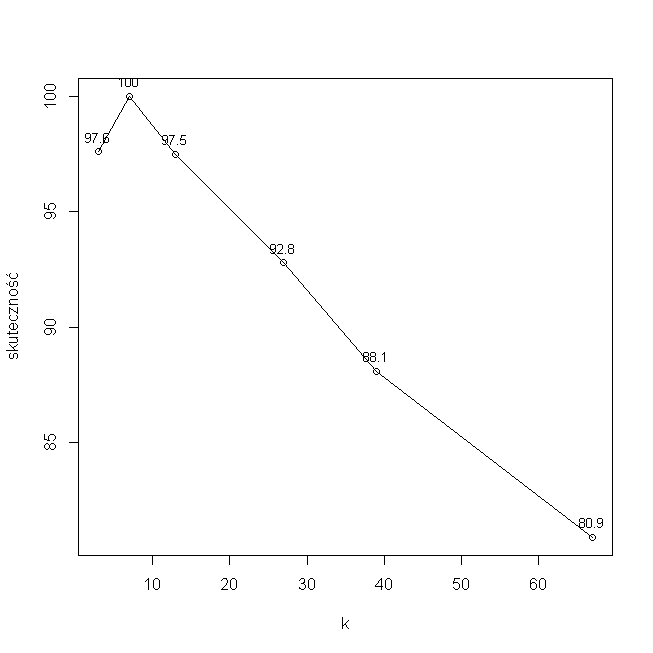
\includegraphics[scale=0.4]{R_knn.png}
 \vspace{-0.1cm}
 \caption{Skuteczność klasyfikacji w \%}
 \label{wykres_k}
\end{figure}

\section{Wnioski}
Poniżej zebrano wnioski wyciągnięte po przedyskutowaniu dokonanych badań. \\

\begin{itemize}
\item{Procent poprawności przewidzenia wyniku dla kolejnej próbki ze zbioru testowego silnie zależy od liczebności zbioru treningowego.}
\item{Zestawie całości zbioru w stosunku 2/3 treningowy, 1/3 testowy dało znacznie lepsze rezultaty od eksperymentów, w których ten stosunek był zamieniony.}
\item{Zbyt mały zbiór danych treningowych może nigdy "nie nauczyć" klasyfikatora rezultatów, których byśmy oczekiwali.}
\item{Jeden z gatunków kwiatów był mocno oddzielony od pozostałych we wszystkich czterech cechach co spowodowało, że algorytm nie miał problemów z jego rozpoznaniem.}
\item{Pozostałe dwa gatunki irysów miały wartości cech bardziej do siebie zbliżone i wtedy wartość współczynnika \textit{k} miała duże znaczenie przy klasyfikacji.}
\item{Współczynnik \textit{k}, czyli ilość najbliższych sąsiadów branych pod uwagę w wyborze klasy próbki, ma bardzo duży wpływ na ogólny wynik.}
\item{Zbyt niska wartość \textit{k} powoduje brak szerszego spojrzenia na otoczenia próbki, co może spowodować przypadkowe przypisanie.}
\item{Zbyt duża wartość \textit{k} może doprowadzić do głosowania wśród większości zbioru testowego i tak naprawdę przekłamywać wynik.}
\item{Bardzo ważne jest wyważenie ilości prób, tak by nie zatrzymać się przy wyniku być może nie dość zadowalającym. Warto jest sprawdzić więcej możliwości niż mniej by mieć większy zbiór danych do analizy.}
\end{itemize}

\addcontentsline{toc}{chapter}{Bibliografia} 
\begin{thebibliography}{99}
\bibitem{zbiory}
Zbiory danych \url{http://archive.ics.uci.edu/ml/}
\bibitem{knn}
Algorytm k-NN \url{http://edu.pjwstk.edu.pl/wyklady/adn/scb/wyklad9/w9.htm}
\bibitem{euklides}
Odległość euklidesowa \url{http://zsi.tech.us.edu.pl/~nowak/ed/PED_kNN.pdf} slajd 8


\end{thebibliography}
\end{document}
